\newcommand{\figureBlinkinLEDGraph}[1]{
  \def\lang{\detokenize{#1}}
  \def\langRu{\detokenize{ru}}
  \def\langEn{en}
  \def\figureCaption{XXX: No translation.}
  \ifx \lang\langRu
  \def\figureCaption{
    Графическое отображение сигнала, меняющегося во времени, на цифровом
    порту.
  }
  \fi
  \if \lang\langEn
  \def\figureCaption{
    Graphical representation of a signal in relation to the time on a
    digital port.
  }
  \fi
  \begin{figure}[ht]
    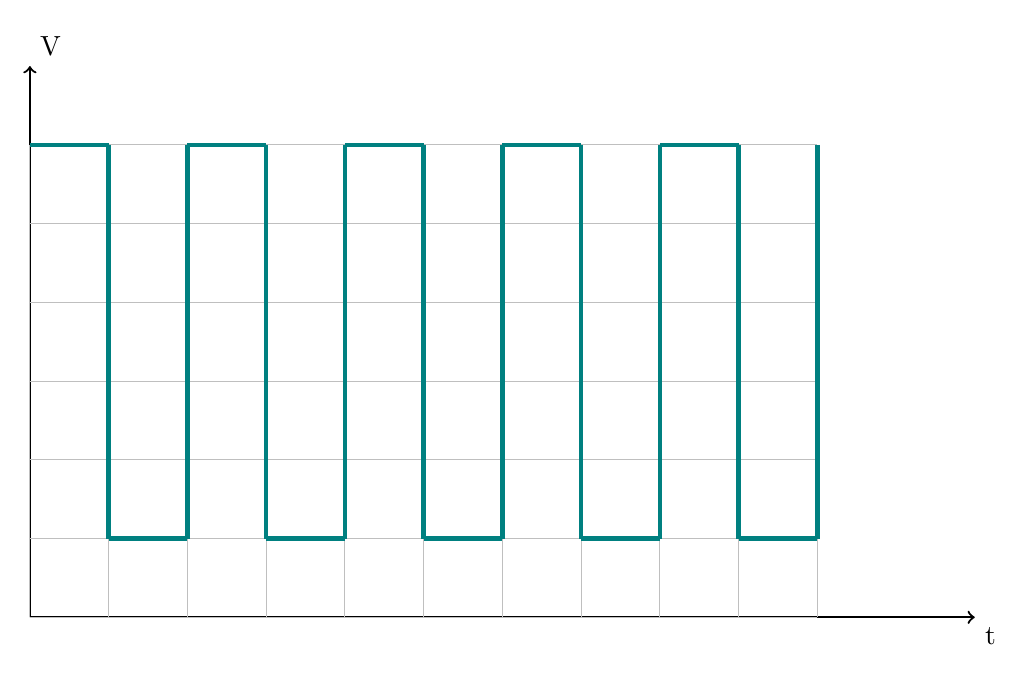
\begin{tikzpicture}
      \draw[thick, ->] (0, 0) -- (12, 0) node[anchor=north west] {t};
      \draw[thick, ->] (0, 0) -- (0,  7) node[anchor=south west] {V};
      \draw[lightgray] (0, 0) grid (10, 6);
      \foreach \x in {0, 2, ..., 8} {
        \draw[ultra thick, teal] (\x, 6) -- (\x + 1, 6);
        \draw[ultra thick, teal] (\x + 1, 6) -- (\x + 1, 1);
        \draw[ultra thick, teal] (\x + 1, 1) -- (\x + 2, 1);
        \draw[ultra thick, teal] (\x + 2, 1) -- (\x + 2, 6);
      }
    \end{tikzpicture}
    \caption{\figureCaption}
    \label{fig:blinking-led-graph}
  \end{figure}
}
